% Dit werk is gelicenseerd onder de licentie Creative Commons Naamsvermelding-GelijkDelen 4.0 Internationaal. Ga naar http://creativecommons.org/licenses/by-sa/4.0/ om een kopie van de licentie te kunnen lezen.
\documentclass[t]{beamer}

\usepackage{amsmath,amsthm}             % Uitgebreide wiskundige mogelijkheden
\usepackage{xcolor}						% Om kleuren te gebruiken

%%%%%%%%%%%%%%%%%%%%%%%%%%%%%%%%%%%%%%%%%%%%%%%%%%%%%%%%%%%%
% Nieuwe commandos
%%%%%%%%%%%%%%%%%%%%%%%%%%%%%%%%%%%%%%%%%%%%%%%%%%%%%%%%%%%%

% De differentiaal operator
\newcommand{\diff}{\ensuremath{\mathrm{d}}}
\newcommand{\subsdiff}{\ensuremath{\mathrm{D}}}
\newcommand{\vardiff}{\ensuremath{\mathrm{\delta}}}

% Super en subscript
\newcommand{\supsc}[1]{\ensuremath{^{\text{#1}}}}   % Superscript in tekst
\newcommand{\subsc}[1]{\ensuremath{_{\text{#1}}}}   % Subscript in tekst

% Vectoren en matrices
\newcommand{\vt}[1]{\ensuremath{\boldsymbol{#1}}} % vector in juiste lettertype
\newcommand{\mx}[1]{\ensuremath{\mathsf{#1}}}	  % matrix in juiste lettertype

% Nieuw commando om iets te benadrukken en tegelijkertijd in de index te steken.
\newcommand{\begrip}[1]{\index{#1}\textbf{#1}\xspace}

% Graden celcius
\newcommand{\degC}{\ensuremath{^\circ \mathrm{C}}}
% graden
\renewcommand{\deg}{\ensuremath{^\circ}}

% unit
\newcommand{\unit}[1]{\ensuremath{\mathrm {#1}}}


% underlinered
\newcommand{\underlinered}[1]{\color{red}\underline{{\color{black}#1}}\color{black}}
%%%%%%%%%%%%%%%%%%%%%%%%%%%%%%
% Packages
%%%%%%%%%%%%%%%%%%%%%%%%%%%%%%

%\usepackage{geometry}              	% 
\usepackage[dutch]{babel}               % Voor nederlandstalige hyphenatie (woordsplitsing)
\uselanguage{dutch}
\languagepath{dutch}
\usepackage{amsmath,amsthm}             % Uitgebreide wiskundige mogelijkheden
\usepackage{url}                        % Om url's te verwerken
\usepackage{graphicx,subfigure}         % Om figuren te kunnen verwerken
\usepackage[utf8]{inputenc}             % Om niet ascii karakters rechtstreeks te kunnen typen
\usepackage[section]{placeins}			% Om ervoor te zorgen dat floats binnen dezelfde section blijven
\usepackage{multicol}
\usepackage[absolute,overlay]{textpos}

%%%%%%%%%%%%%%%%%%%%%%%%%%%%%%
% Layout
%%%%%%%%%%%%%%%%%%%%%%%%%%%%%%
\usetheme{Frankfurt}
\usefonttheme[onlymath]{serif}
\AtBeginSection[]
{
  \begin{frame}
    \frametitle{Inhoud}
    \tableofcontents[currentsection]
  \end{frame}
}

\setbeamertemplate{navigation symbols}{}
\setbeamertemplate{footline}[page number]

%%%%%%%%%%%%%%%%%%%%%%%%%%%%%%
% Title
%%%%%%%%%%%%%%%%%%%%%%%%%%%%%%
\title{Fluïdummechanica}
\author{Brecht Baeten\inst{1}}
\institute{
	\inst{1}%
  		KU Leuven, Technologie campus Diepenbeek,\\ e-mail: brecht.baeten@kuleuven.be
}
\date{\today}
%%%%%%%%%%%%%%%%%%%%%%%%%%%%%%
% Omgevingen
%%%%%%%%%%%%%%%%%%%%%%%%%%%%%%


\subtitle{Open kanaalstroming}

\begin{document}

	\frame{\titlepage}
%%%%%%%%%%%%%%%%%%%%%%%%%%%%%%%%%%%%%%%%%%%%%%%%%%%%%%%%%%%%%%%%%%%%%%%%%%%
	\section{Inleiding}
	\begin{frame}
		\frametitle{Voorbeeld}
		\center
		\vspace{-0.5cm}
    	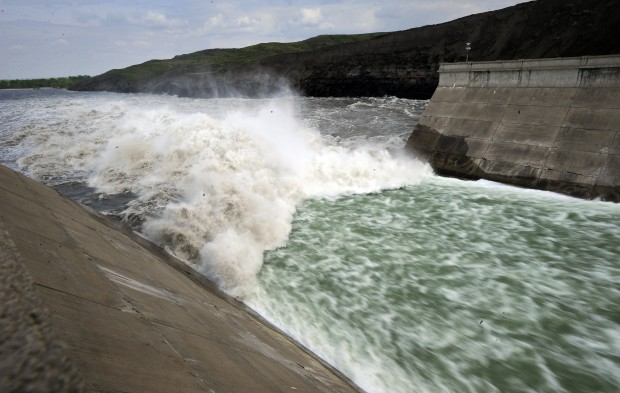
\includegraphics[width=\textwidth]{../fig/kanaalstroming/Fort_Peck_Dam_spillway.jpg}\\
    	\footnotesize{Bron: http://billingsgazette.com/}
  	\end{frame}
%%%%%%%%%%%%%%%%%%%%%%%%%%%%%%%%%%%%%%%%%%%%%%%%%%%%%%%%%%%%%%%%%%%%%%%%%%%
  	\begin{frame}
  		\frametitle{Doorsnedes}
		\center
		\only<1-2>{
			\vspace{1cm}		
			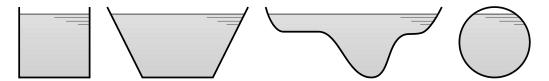
\includegraphics[width=\textwidth]{../fig/kanaalstroming/Open_kanaal_doorsnedes}\\
		}
		\only<2>{
			\vspace{2cm}
			Het oppervlak is vrij om te vervormen
		}
  	\end{frame}
%%%%%%%%%%%%%%%%%%%%%%%%%%%%%%%%%%%%%%%%%%%%%%%%%%%%%%%%%%%%%%%%%%%%%%%%%%%
	\section{Oppervlaktegolven}	
	\begin{frame}
		\frametitle{Golfsnelheid}
		\only<1>{
			\center
			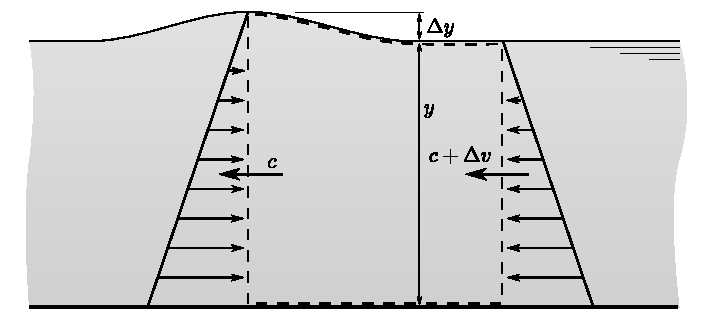
\includegraphics[width=\textwidth]{../fig/kanaalstroming/Golfsnelheid}
		}
		\only<2-8>{
			\begin{textblock}{5}(0,3)
            	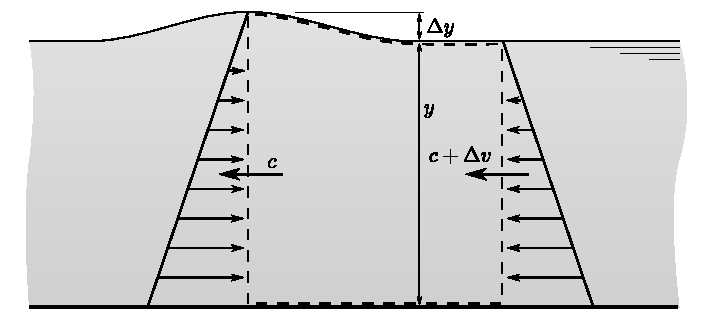
\includegraphics[width=5cm]{../fig/kanaalstroming/Golfsnelheid}
       		\end{textblock}
       		\vspace{2.5cm}
		}
		\only<2-3>{
			Behoud van massa:
			\begin{equation*}
				0 = (c+\Delta v) b y - c b (y+\Delta y)
			\end{equation*}
		}
		\only<3-3>{
			\begin{equation}
				c = y \frac{\Delta v}{\Delta y}
				\label{eqn:golfsnelheid behoud van massa}
			\end{equation}
		}
		\refstepcounter{equation}
		\only<4-6>{
			Behoud van impuls:
			\begin{equation*}
				\frac{1}{2}\rho g (y+\Delta y)^2 b - \frac{1}{2}\rho g y^2 b = \rho b (y+\Delta y) c (c+\Delta v-c)
			\end{equation*}
		}
		\only<5-6>{
			\begin{equation*}
	 			g \left(\frac{y}{\Delta y} + \frac{1}{2}\right)  = c \left(\frac{y}{\Delta y} + 1\right)\frac{\Delta v}{\Delta y}
			\end{equation*}
		}
		\only<6-6>{
			\begin{equation}
				\dfrac{\Delta v}{\Delta y} = \dfrac{g}{c} \dfrac{\dfrac{y}{\Delta y} + \frac{1}{2}}{\dfrac{y}{\Delta y} + 1} \approx \dfrac{g}{c}
				\label{eqn:golfsnelheid behoud van impuls}
			\end{equation}
		}
		\refstepcounter{equation}
		\only<7-8>{
			% Latex equation labeling and numbering seems not to work inside only environments
			(1) en (2):	
			\begin{align*}
				c &= y \frac{\Delta v}{\Delta y} \\
				\dfrac{\Delta v}{\Delta y} &\approx \dfrac{g}{c}
			\end{align*}
		}
		\only<8-8>{
			\vspace{0.5cm}
			\begin{equation}
				c = \sqrt{g y}
				\label{eqn:golfsnelheid ondiep}
			\end{equation}
		}
		\refstepcounter{equation}
  	\end{frame}
%%%%%%%%%%%%%%%%%%%%%%%%%%%%%%%%%%%%%%%%%%%%%%%%%%%%%%%%%%%%%%%%%%%%%%%%%%%
	\section{Specifieke energie diagram}	
	\begin{frame}
		\frametitle{Bernoulli}
		\only<1>{
			\center
			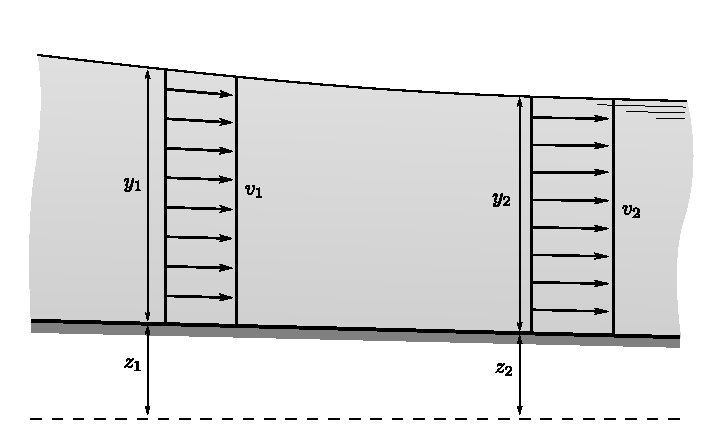
\includegraphics[width=\textwidth]{../fig/kanaalstroming/Open_kanaal_bernoulli_zonder_energielijn}
		}
		\only<2-3>{
			\begin{textblock}{5}(0,3)
            	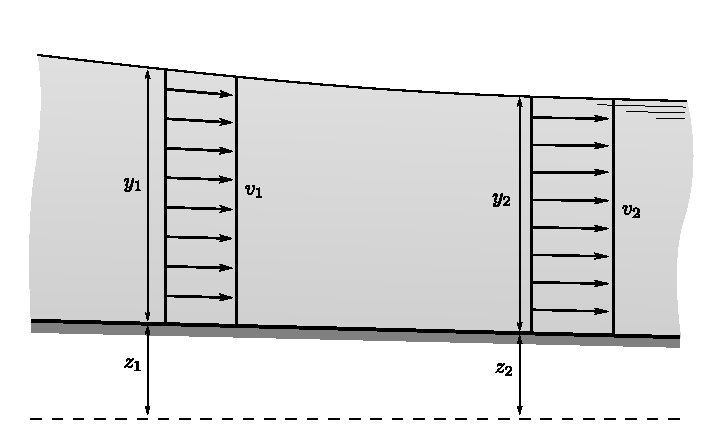
\includegraphics[width=5cm]{../fig/kanaalstroming/Open_kanaal_bernoulli_zonder_energielijn}
       		\end{textblock}
       		\vspace{2.5cm}
		}
		\only<2-3>{
			\vspace{1cm}
			\begin{equation*}
				\frac{p_1}{\rho g} + \frac{v_1^2}{2 g} + z_1 = \frac{p_2}{\rho g} + \frac{v_2^2}{2 g} + z_2
			\end{equation*}
		}
		\only<3-3>{
			\vspace{0.5cm}
			\begin{equation*}
				y_1 + \frac{v_1^2}{2 g} + z_1 = y_2 + \frac{v_2^2}{2 g} + z_2
			\end{equation*}
		}
		\only<4>{
			\center
			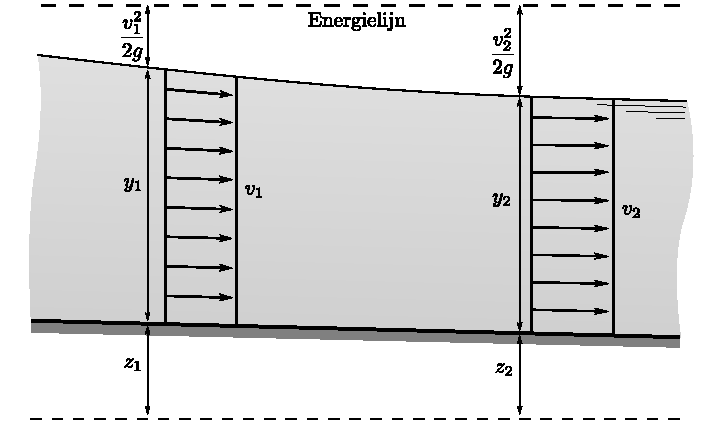
\includegraphics[width=\textwidth]{../fig/kanaalstroming/Open_kanaal_bernoulli}
		}
  	\end{frame}
%%%%%%%%%%%%%%%%%%%%%%%%%%%%%%%%%%%%%%%%%%%%%%%%%%%%%%%%%%%%%%%%%%%%%%%%%%%
	\begin{frame}
		\frametitle{Specifieke energie}
		\only<1-3>{
			\begin{textblock}{5}(0,3)
            	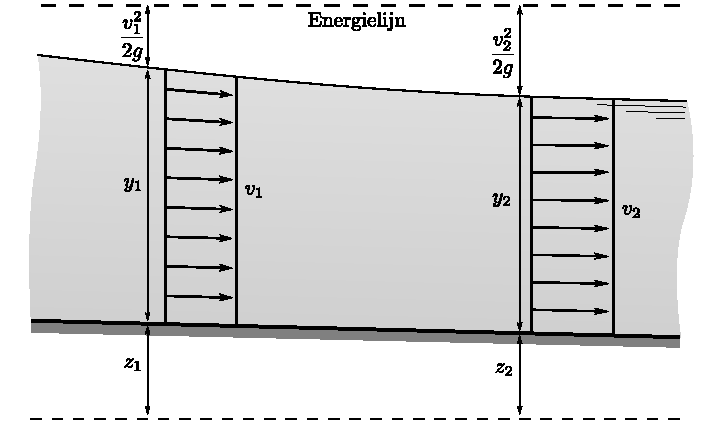
\includegraphics[width=5cm]{../fig/kanaalstroming/Open_kanaal_bernoulli}
       		\end{textblock}
       		\vspace{3cm}
		}
		\only<1-1>{
			\begin{equation*}
				y_1 + \frac{v_1^2}{2 g} + z_1 = y_2 + \frac{v_2^2}{2 g} + z_2
			\end{equation*}
		}
		\only<2-3>{
			\begin{equation*}
				\underlinered{y_1 + \frac{v_1^2}{2 g}} + z_1 = \underlinered{y_2 + \frac{v_2^2}{2 g}} + z_2
			\end{equation*}
		}
		\only<2-3>{
			\begin{equation*}
				E = y + \frac{v^2}{2 g}
			\end{equation*}
			\begin{equation*}
				E_1 + z_1 = E_2 + z_2
			\end{equation*}
		}
		\only<3-3>{
			\center
			\vspace{0.2cm}
			Op een gegeven locatie kan enkel de specifieke energie $E$ variëren
		}
  	\end{frame}
%%%%%%%%%%%%%%%%%%%%%%%%%%%%%%%%%%%%%%%%%%%%%%%%%%%%%%%%%%%%%%%%%%%%%%%%%%%
	\begin{frame}
		\frametitle{Specifieke energie diagram}
		\only<1-4>{
			\begin{equation*}
				E = y + \frac{v^2}{2 g}
			\end{equation*}
		}
		\only<2-4>{
			De hoogte en de snelheid in een kanaal zijn niet onafhankelijk:
			\begin{equation*}
				\dot{V} = v y b
			\end{equation*}
		}
		\only<3-4>{
			\begin{equation*}
				E = y + \frac{\dot{V}^2/b^2}{2 g y^2}
			\end{equation*}
		}
		\only<4-4>{
			Met het debiet per eenheid breedte, $q$:
			\begin{equation*}
				E = y + \frac{q^2}{2 g y^2}
			\end{equation*}
		}
		\only<5>{
			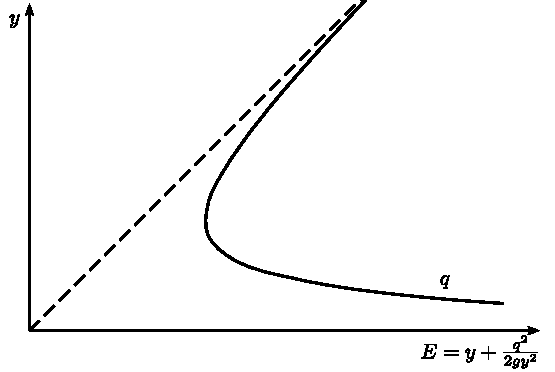
\includegraphics[width=\textwidth]{../fig/kanaalstroming/Specifieke_energie_diagram_enkel}
		}
		\only<6>{
			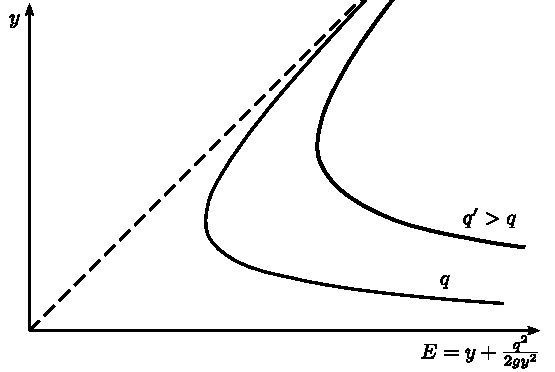
\includegraphics[width=\textwidth]{../fig/kanaalstroming/Specifieke_energie_diagram_groter_debiet}
		}
  	\end{frame}
%%%%%%%%%%%%%%%%%%%%%%%%%%%%%%%%%%%%%%%%%%%%%%%%%%%%%%%%%%%%%%%%%%%%%%%%%%%
	\section{Stromingstypes}
	\begin{frame}
		\frametitle{Kritische stroming}
		\only<1>{
			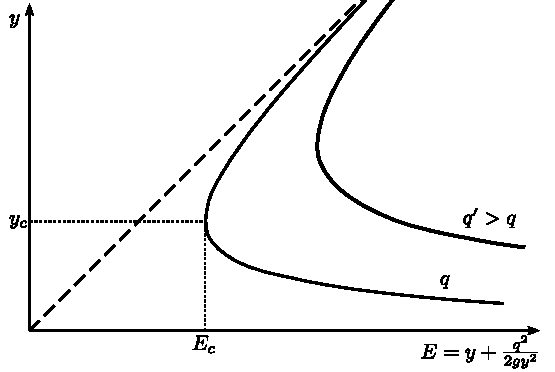
\includegraphics[width=\textwidth]{../fig/kanaalstroming/Specifieke_energie_diagram_kritisch}
		}
		\only<2-5>{
			\begin{textblock}{5}(0,3)
            	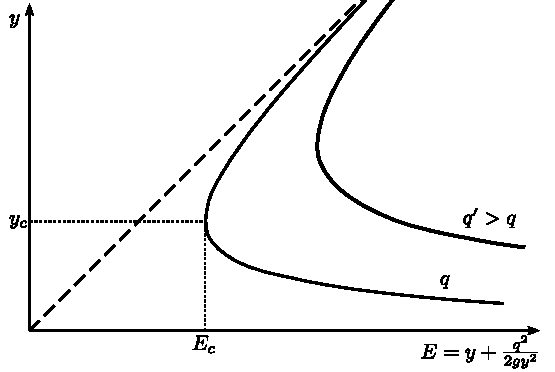
\includegraphics[width=4.5cm]{../fig/kanaalstroming/Specifieke_energie_diagram_kritisch}
       		\end{textblock}
       		\vspace{3cm}
		}
		\only<2-5>{
			\begin{equation*}
				\frac{\diff E}{\diff y} = 1 - \frac{q^2}{g y^3} = 0
			\end{equation*}
		}
		\only<3-5>{
			\begin{equation*}
				y_c = \left( \frac{q^2}{g} \right)^{1/3}
			\end{equation*}
		}
		\only<4-5>{
			\begin{equation*}
				v_c = \sqrt{g y_c}
			\end{equation*}
		}
		\only<5-5>{
			\center
			Bij kritische stroming is de snelheid gelijk aan de golfsnelheid
		}
  	\end{frame}
%%%%%%%%%%%%%%%%%%%%%%%%%%%%%%%%%%%%%%%%%%%%%%%%%%%%%%%%%%%%%%%%%%%%%%%%%%%
	\begin{frame}
		\frametitle{Stromingstypes}
		\only<1-4>{
			\begin{center}
				Snelheid kleiner dan de golfsnelheid:\\
				\emph{Subkritische stroming}
			\end{center}
		}
		\only<2-4>{
			\begin{center}
				Snelheid groter dan de golfsnelheid:\\
				\emph{Superkritische stroming}
			\end{center}
		}
		\only<3-4>{
			Dimensieloze uitdrukking:
			\begin{equation*}
				\mathrm{Fr} = \frac{v}{c} = \frac{v}{\sqrt{g y}}
			\end{equation*}
		}
		\only<4-4>{
			\vspace{-0.5cm}
			\begin{align*}
				\mathrm{Fr} &= 1 \qquad  \text{Kritische stroming}\\
				\mathrm{Fr} &< 1 \qquad  \text{Subkritische stroming}\\
				\mathrm{Fr} &> 1 \qquad  \text{Superkritische stroming}
			\end{align*}
		}
		\only<5-5>{
			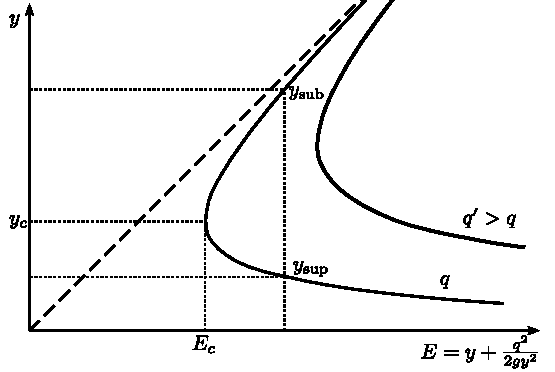
\includegraphics[width=\textwidth]{../fig/kanaalstroming/Specifieke_energie_diagram}
		}
  	\end{frame}
%%%%%%%%%%%%%%%%%%%%%%%%%%%%%%%%%%%%%%%%%%%%%%%%%%%%%%%%%%%%%%%%%%%%%%%%%%%
	\begin{frame}
		\frametitle{Veranderingen in de bodem}
		\only<1>{
			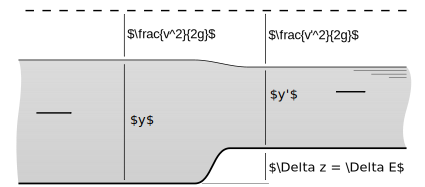
\includegraphics[width=\textwidth]{../fig/kanaalstroming/Open_kanaal_bodemstijging_subkritisch}
		}
		\only<2>{
			\center
            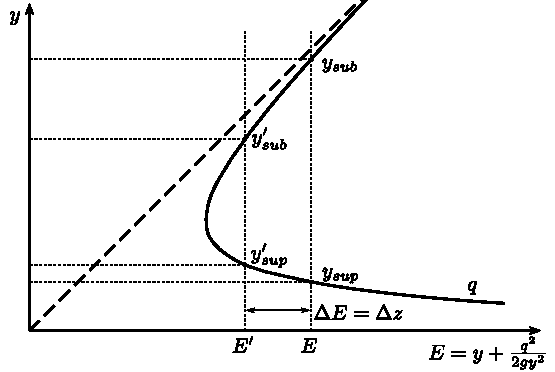
\includegraphics[width=\textwidth]{../fig/kanaalstroming/Specifieke_energie_diagram_bodemstijging}
       	}
       	\only<3>{
			\noindent
			\begin{columns}[t,onlytextwidth]
				\column{.50\textwidth}
					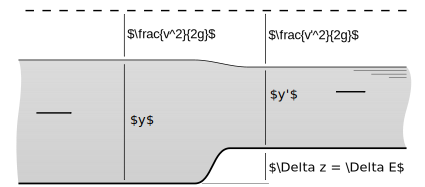
\includegraphics[width=\textwidth]{../fig/kanaalstroming/Open_kanaal_bodemstijging_subkritisch}
				\column{.50\textwidth}
					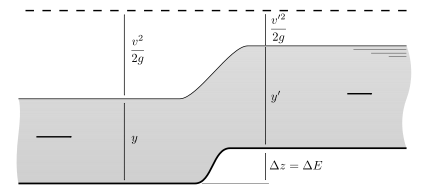
\includegraphics[width=\textwidth]{../fig/kanaalstroming/Open_kanaal_bodemstijging_superkritisch}
			\end{columns}
			
			\center
            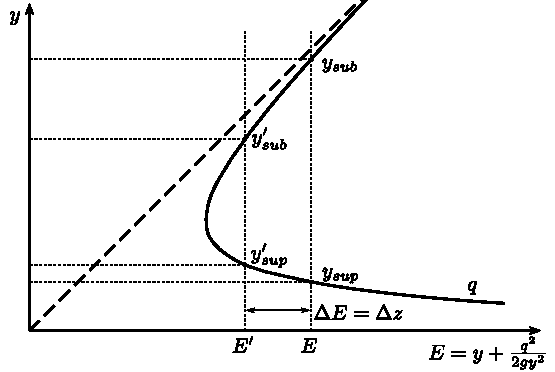
\includegraphics[width=0.6\textwidth]{../fig/kanaalstroming/Specifieke_energie_diagram_bodemstijging}
		}
  	\end{frame}
%%%%%%%%%%%%%%%%%%%%%%%%%%%%%%%%%%%%%%%%%%%%%%%%%%%%%%%%%%%%%%%%%%%%%%%%%%%
	\begin{frame}
		\frametitle{Overgangen tussen stromingstypes}
		\only<1>{
			\vspace{1cm}
			\center
			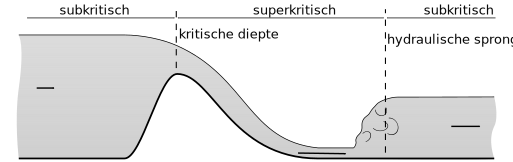
\includegraphics[width=\textwidth]{../fig/kanaalstroming/Open_kanaal_subkritisch_naar_superkritisch}
		}
		\only<2>{
			\center
    		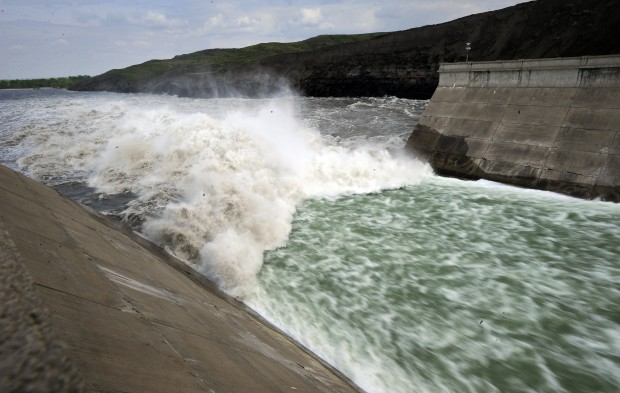
\includegraphics[width=\textwidth]{../fig/kanaalstroming/Fort_Peck_Dam_spillway.jpg}\\
    		\footnotesize{Bron: http://billingsgazette.com/}
		}
	\end{frame}
%%%%%%%%%%%%%%%%%%%%%%%%%%%%%%%%%%%%%%%%%%%%%%%%%%%%%%%%%%%%%%%%%%%%%%%%%%%
	\section{Analogie met samendrukbare stroming}
	\begin{frame}
		\frametitle{Samendrukbare stroming}
		\only<1-5>{
			In een samendrukbare stroming kunnen drukgolven ontstaan
		
			De voortplantingssnelheid is de snelheid van het geluid $c$
		}
		\only<2-5>{
			\begin{equation*}
				\mathrm{Ma} = \frac{v}{c}
			\end{equation*}
		}
		\only<3-5>{
			\vspace{-0.4cm}
			
			$\mathrm{Ma} < 1$, Subsone stroming:\\
			Verkleinen van de doorstroom opening zal de snelheid doen stijgen
		}
		\only<4-5>{
			
			$\mathrm{Ma} > 1$, Supersone stroming:\\
			Vergroten van de doorstroom opening zal de snelheid doen stijgen
		}
		\only<5-5>{
		
			\vspace{0.6cm}
			\centering
			Convergerend - divergerend nozzle om een stroming tot boven de geluidssnelheid te versnellen\\
			Overgang van supersone naar subsone stroming gaat gepaard met een schokgolf
		}
		\only<6>{
			\vspace{0.5cm}
			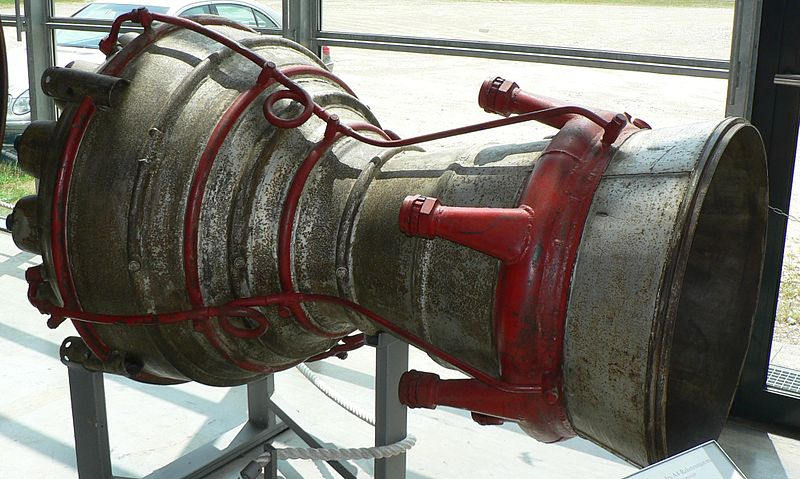
\includegraphics[width=\textwidth]{../fig/kanaalstroming/v2_rocket_nozzle.jpg}
		}
		\only<7>{
			\vspace{1cm}
			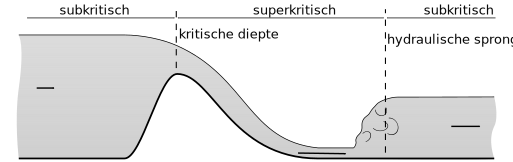
\includegraphics[width=\textwidth]{../fig/kanaalstroming/Open_kanaal_subkritisch_naar_superkritisch}
		}
  	\end{frame}
%%%%%%%%%%%%%%%%%%%%%%%%%%%%%%%%%%%%%%%%%%%%%%%%%%%%%%%%%%%%%%%%%%%%%%%%%%%
\end{document}